\documentclass[a4paper,14pt]{extarticle}
\usepackage{geometry}
\usepackage[T1]{fontenc}
\usepackage[utf8]{inputenc}
\usepackage[main=english, russian]{babel}   % use russian via \foreignlanguage{russian}{}
\usepackage{amsmath}
\usepackage{amsthm}
\usepackage{amssymb}
\usepackage{fancyhdr}
\usepackage{setspace}
\usepackage{graphicx}
\usepackage{colortbl}
\usepackage{tikz}
\usepackage{pgf}
\usepackage{subcaption}
\usepackage{listings}
\usepackage{indentfirst}
\usepackage[colorlinks,citecolor=blue,linkcolor=blue,bookmarks=false,hypertexnames=true, urlcolor=blue]{hyperref} 
\usepackage{indentfirst}
\usepackage{mathtools}
\usepackage{booktabs}
\usepackage[flushleft]{threeparttable}
\usepackage{tablefootnote}

\usepackage{chngcntr} % нумерация уравнений, графиков и таблиц по секциям
\counterwithin{equation}{section}
\counterwithin{table}{section}
\counterwithin{figure}{section}

% \graphicspath{{graphics/}}%путь к рисункам     You may leave it

% add bibliography using biblatex
% if if all authors in bibliography are needed => add 'maxbibnames=99' in []:
\usepackage[backend=biber, citestyle=authoryear]{biblatex}
\addbibresource{bibliography.bib}
\DeclareFieldFormat{labelnumberwidth}{#1\adddot}
\setlength{\biblabelsep}{5pt}
 

\geometry{left=2.5cm}% левое поле
\geometry{right=1.5cm}% правое поле
\geometry{top=1.5cm}% верхнее поле
\geometry{bottom=1.5cm}% нижнее поле
\renewcommand{\baselinestretch}{1.5} % междустрочный интервал


\renewcommand{\theenumi}{\arabic{enumi}}% Меняем везде перечисления на цифра.цифра
\renewcommand{\labelenumi}{\arabic{enumi}}% Меняем везде перечисления на цифра.цифра
\renewcommand{\theenumii}{.\arabic{enumii}}% Меняем везде перечисления на цифра.цифра
\renewcommand{\labelenumii}{\arabic{enumi}.\arabic{enumii}.}% Меняем везде перечисления на цифра.цифра
\renewcommand{\theenumiii}{.\arabic{enumiii}}% Меняем везде перечисления на цифра.цифра
\renewcommand{\labelenumiii}{\arabic{enumi}.\arabic{enumii}.\arabic{enumiii}.}% Меняем везде перечисления на цифра.цифра

\begin{document}
\begin{titlepage}
\newpage

{\setstretch{1.0}
\begin{center}
Federal State Autonomous Educational Institution for Higher Education
National Research University Higher School of Economics
\\
\bigskip
Faculty of Computer Science \\
Applied Mathematics and Information Science \\
\end{center}
}

\vspace{8em}

\begin{center}
{\Large BACHELOR'S THESIS}\\
\textsc{\textbf{
Research project
\linebreak
"Your Theme"}}
\end{center}

\vspace{4em}

{\setstretch{1.0}
\hfill\parbox{16cm}{
\hspace*{5cm}\hspace*{-5cm}Prepared by the student of group 171, 4th year of study,\\
Gelvan Kirill Pavlovich\\

\hspace*{5cm}\hspace*{-5cm}Supervisor:\\
Senior Research Fellow, Nadezhda Chirkova
\\

\hspace*{5cm}\hspace*{-5cm}Curator:\\
...\\

\hspace*{5cm}\hspace*{-5cm}Consultant:\\
...\\
}
}

\vspace{\fill}

\begin{center}
Moscow 2021
\end{center}

\end{titlepage}
% это титульный лист
\newpage

{
	\hypersetup{linkcolor=black}
	\tableofcontents
}

\newpage
\section*{Annotation} 
\addcontentsline{toc}{section}{Annotation}  % add Annotation to Table of Contents

Your annotation in English.

\section*{\foreignlanguage{russian}{Аннотация}}   % this is how to use russian
\foreignlanguage{russian}{
    Ваша аннотация на русском языке.
}

\section*{Keywords}
NLP, CV, DL, ML, RL, GAN, 
\pagebreak

\section{Introduction}

\subsection{Citing}

In this template you have to insert all your references in a special file 
called "bibliography.bib". It should be inserted in a special BibTex format. 
It can be found easily via google scholar -> quotation sign -> BibTex. You can find how it looks in ".bib" file.

After you have inserted your BibTex citation into the ".bib" file, you can cite it in this document using \cite{vaswani2017}.

\subsection{Graphs}

Graph \ref{fig:by_epochs} is useless.

\begin{figure}[h!]
	\centering
	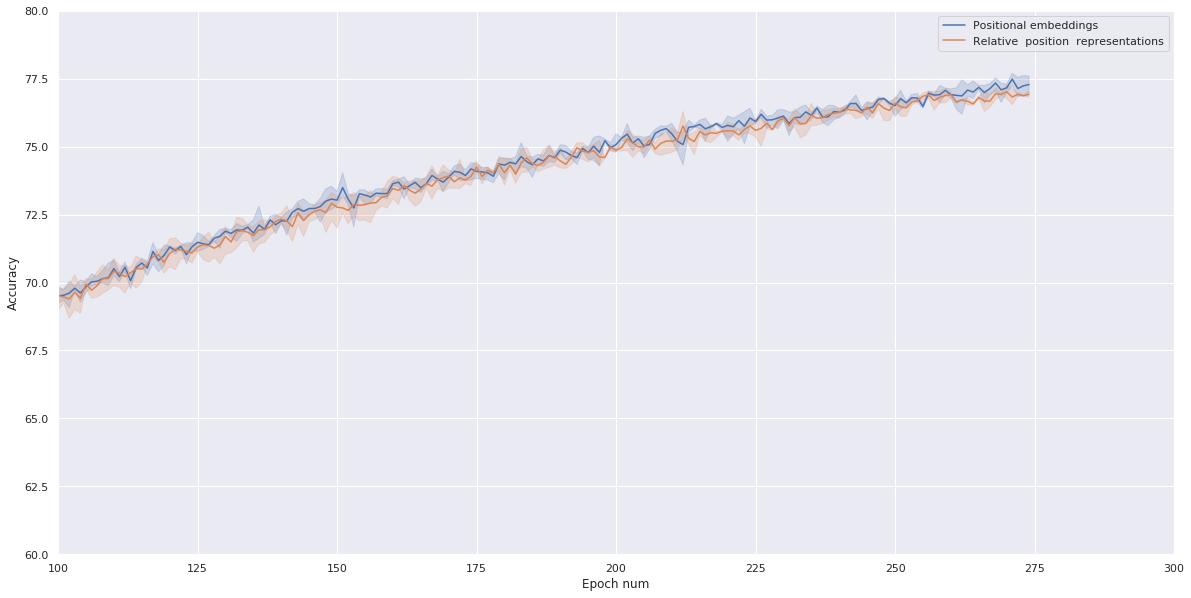
\includegraphics[width=1\textwidth]{graph2.png}
	\caption{Graph sample}
	\label{fig:by_epochs}
\end{figure}

\pagebreak

\subsection{Tables}

\begin{table}[htbp]
	\caption{Table example}
	\label{table:long_epochs}
	\footnotesize
	\centering
	\begin{tabular}{lrrrrrrrr}
		\toprule
		& \multicolumn{3}{c}{$\mathsf{Val}$} &
		\multicolumn{3}{c}{$\mathsf{Test}$} \\
		\cmidrule(lr){2-4} \cmidrule(l){5-7} 
		{} &  $\mathsf{Prec}$ &  $\mathsf{Rec}$ &  $\mathsf{F1}$ &  $\mathsf{Prec}$ &  $\mathsf{Rec}$ &  $\mathsf{F1}$  &  $\mathsf{nodes}$ & $\mathsf{subtokens}$\\
		\midrule
		run 1    &    0.4894 &   0.3775 &  0.4263 &     0.4824 &    0.3683 &   0.4177 & 10029 & 179\\
		run 2    &    0.4887 &   0.3739 &  0.4237 &     0.4891 &    0.3724 &   0.4228 & 10039 & 177\\
		run 3    &    0.4820 &   0.3751 &  0.4219 &     0.4838 &    0.3677 &   0.4178 & 10037&	180\\
		\midrule
		\bf{mean} &    \bf{0.4867} &   \bf{0.3755} &  \bf{0.4239} &    \bf{ 0.4851} &    \bf{0.3695} &   \bf{0.4195} \\
		\bf{variance}  &    0.0041 &   0.0019 &  0.0022 &     0.0036 &    0.0025 &   0.0029 \\
		\bottomrule
	\end{tabular}
\end{table}

	
\newpage 

% 1 command to write all citations into the References
\printbibliography[heading=bibintoc]   % [] are for appearing in Table of Contents
	
\end{document}
